%%% Extra:
\textbf{Hasta 1.5pts extra.} Determina el código de tres direcciones
de la siguiente expresión,
\begin{center}
   $(a \ SUB \ b ) \ MOD \ ((MINUS \ c)  \ SUB \ d)$
\end{center}
usando las reglas semánticas siguientes. \\
Pueden omitir la explicación de la creación del árbol de sintaxis abstracta, 
pero hay que explicar los pasos del análisis semántico.

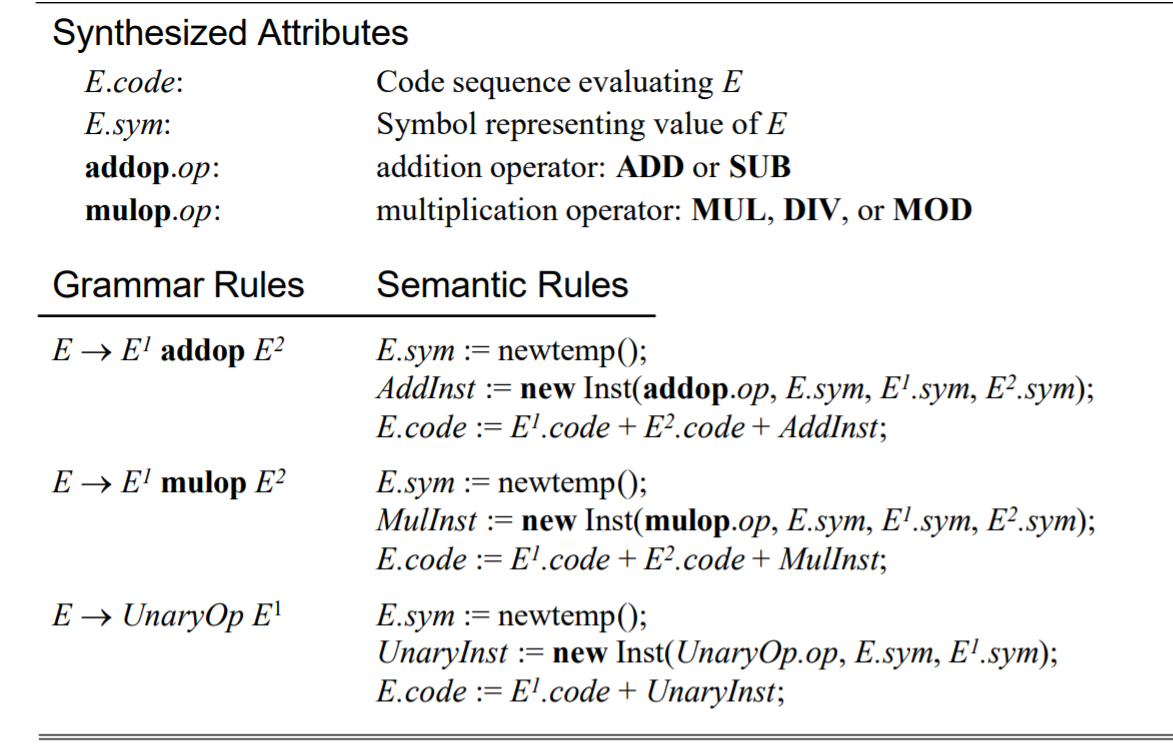
\includegraphics[width=0.7\linewidth]{./Fun_Sem_1.PNG}

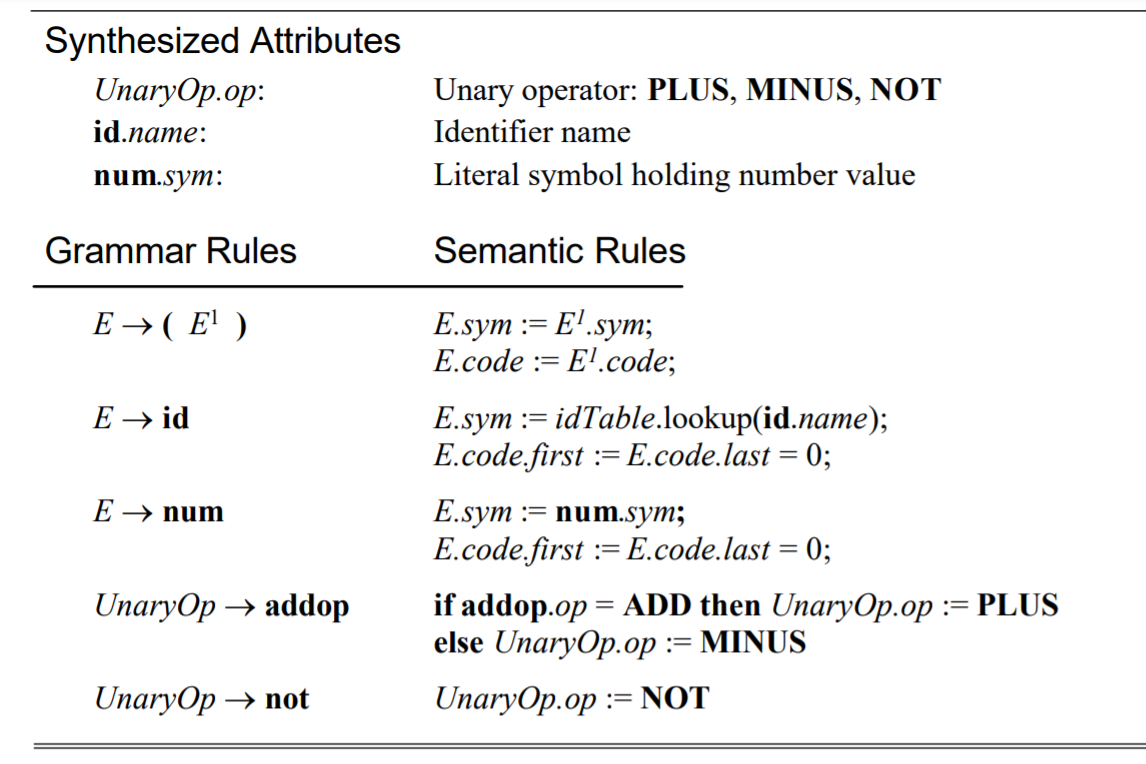
\includegraphics[width=0.7\linewidth]{./Funciones_Semanticas_2.PNG}

\textbf{Solución:} A continuación se muestra el código en tres direcciones
para la expresión dada

\begin{center}
\begin{tabular}{c | c}
Código 3 direcciones & Reglas Semánticas\\ \hline
$t_1 = a - b$        & $E \rightarrow (E^1) \rightarrow (E^{11} \text{ addop } E^{12}) \rightarrow (E^{11}.\text{sym} \text{ addop.op } E^{12}.\text{sym}) \rightarrow  (id.name \text{ SUB } id.name)$ \\
$t_2 = - c$          & $E \rightarrow (E^1) \rightarrow (\text{ UnaryOp } E^{11}) \rightarrow (\text{ MINUS } E^{11}.\text{sym}) \rightarrow (\text{ MINUS } id.name)$ \\
$t_3 = t_2 - d$      & $E \rightarrow (E^1) \rightarrow (E^{11} \text{ addop } E^{12}) \rightarrow (E^{11}.\text{sym} \text{ addop.op } E^{12}.\text{sym}) \rightarrow  (id.name \text{ SUB } id.name)$ \\
$t_4 = t_1 \mod t_3$ & $E \rightarrow (E^1) \rightarrow (E^{11} \text{ addop } E^{12}) \rightarrow (E^{11}.\text{sym} \text{ addop.op } E^{12}.\text{sym}) \rightarrow  (id.name \text{ MOD } id.name)$
\end{tabular} 
\end{center}
